\documentclass[12pt]{report}
\usepackage[utf8]{inputenc}
\usepackage[T1]{fontenc}
\usepackage[english]{babel}
\linespread{1.50}

\usepackage{geometry}
 \geometry{
 a4paper,
 total={170mm,257mm},
 left=40mm,
 right=40mm,
 top=20mm,
 bottom=30mm,
 }

%%% Bibliography
\usepackage[square,numbers]{natbib}
\usepackage{url}
\usepackage{hyperref}
\bibliographystyle{abbrvnat}


%%% Grafik
\usepackage{epstopdf}
\usepackage{graphicx}
\usepackage{float}

%%% math
\usepackage{amsmath}
\usepackage{amsfonts}
\usepackage{amssymb}
\usepackage[amssymb]{SIunits}
\usepackage{units}
%%% Kode
\usepackage{listings}

%%% TABLES
\usepackage{tabularx}
\usepackage{booktabs}

%%% Farve formaterring 
\usepackage{color}

%%% Dokument miljø 

\title{P1 Project - Computer Science\\Package delivery}
\author{\textbf{Aalborg university - Group A325}\\Alexander Pihl Stückler\\Casper Munk\\Morten Madsen\\Niklas Jespersgaard Bruun\\Nikolaj Müller larsen\\Simon Kanne Mikkelsen\\Simon Kingo Møller}
\date{October-December 2018}

\begin{document}

\maketitle

\tableofcontents


\chapter{Introduction}
Usage of the internet for online shopping is steadily growing among people around the world\cite{FDIHyearreport}. A large part of these online purchases requires packages to be delivered and the companies responsible for delivering said packages have a lot of different methods of ensuring safe and quick delivery\cite{postnordoptions, glsoptions, upsoptions}. These methods revolves around the well known Travelling Salesman Problem and the complex algorithms within\cite{tsp}. Having fully optimized routes could save a company a lot of money and ensure that packages gets delivered in first attempt. 



\section{The initial problem}
In this section the initial problem is presented and it will be the foundation for this report. The initial problem consists of one main problem and three sub questions to which will be answered in order to narrow down the problem field. \\

There are many different problems in package delivery that could be improved upon. However there seems to be a general interest in improving customer satisfaction. It would be interesting to investigate how to optimize the delivery system in a way that would benefit the end customer.
\\

\textbf{Main problem:}\\
Failed delivery attempts due to recipients not being home. \\

\textbf{Sub questions:}
\begin{itemize}
\item Is this a real problem?
\item Is it beneficial for companies to focus on customer satisfaction?
\item How does existing methods handle similar problems?
\end{itemize}


\chapter{Problem analysis}
This problem analysis seeks to answer the sub-questions listed in the initial problem to further understand the main problem. Answering these questions creates understanding for the problem and helps with narrowing the problem field. \\\hspace*{5 mm}
By looking at who the typical customer is and how they prefer to get their packages delivered. Can this information be used to conduct a survey which can be used to find tendencies in cases of problems and solutions associated with package delivery. \\\hspace*{5 mm}
It would then be interesting to examine if the delivery companies benefits from prioritizing customer satisfaction even if this means a loss in income. Finally, the current methods of handling certain relevant problems will be studied and the information obtained will be used to find a real problem that can be solved or optimized in a way that would benefit the end customer.



%SUB QUESTION 1: Is this a real problem?

\section{Growth in package delivery in correlation to online shopping}
%Er nu omskrevet, og skal læses igennem.
The increased popularity of the internet has made it more accessible for people to order packages from all over the world. In 2017, 80\% of Danes have used online shopping within the last year, When it only was 59\% in 2008 \cite{Ehandel2017}. \\\hspace*{5 mm}
E-commerce is a term used to describe any type of online transactions. That means that e-commerce involves both physical and digital product. The term is widely used in business analysis to get a better understanding of the general growth in online shopping. Danish E-commerce Association (FDIH) is an industry association that wants to help companies that primarily focus on online shopping \cite{fdihabout}. They have a lot of statistics about e-commerce because of that. Statistic that can be useful to determine the growth in both e-commerce and more importantly package delivery. \\\hspace*{5 mm}
According to FDIH's year report for 2017, a total of 176 million e-commerce were made which is an increase of 9\% compared to 2016. 75\% of these trades involved physical products that in some way needed shipping.\cite{FDIHyearreport}. It can then be assumed that online shopping have a large influence on the total amount of packages delivered each year.
From these statistic its safe to assume that online shopping keeps growing which also means a growth in package delivery.%-slutning-




\section{Frequent users of online shopping}
%Skal læses igennem, måske omskrives lidt i den sidste del.
It is established in the previous section that the amount of people who purchases online is gradually increasing every year and a large part of these e-commerce involves package delivery. This section focuses on the different age groups that use the internet for shopping.

\begin{figure}[H]
  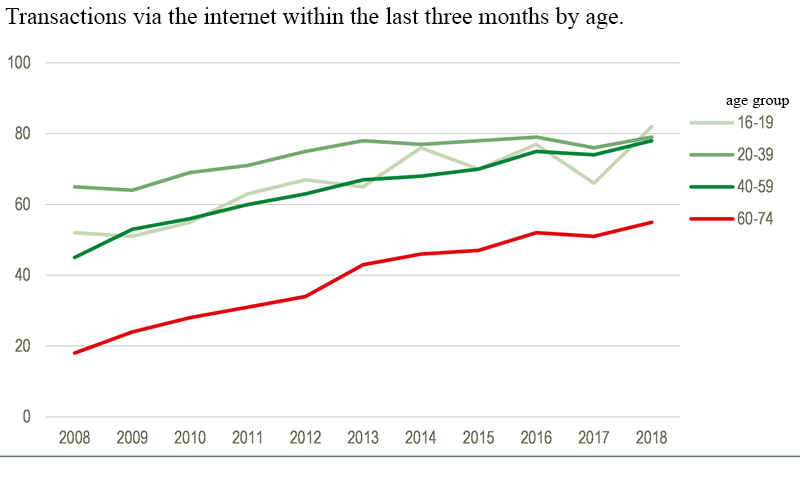
\includegraphics[width=\linewidth]{pics/customer.png}
  \caption{Age groups over time. \cite{danmarkstat2}}
  \label{fig:Agegroupsovertime}
\end{figure}

Statistics Denmark (DST) have made statistic surrounding this.
 It shows that 82\% of people in Denmark between ages 16 and 19 have been online shopping within the last 3 months in 2018. While the age groups from 20 to 39 years and 40 to 59 years sits at 79\% and 78\% respectively, see Figure \ref{fig:Agegroupsovertime}. 55\% of elders between 60 and 74 years have used online shopping in last three months which may seem like a small amount compared to the younger age groups, but the elders have increased their online shopping more than any other age group. In 2008 they were only at 18\% which means an increase of 37\% within the last 10 years \cite{danmarkstat1}.
While the statistics does not show a big difference in the the two younger age groups covering ages 16 to 59, it does show that younger people tend use the internet for shopping more frequently. \\
statistics done by DST from 2015\cite{DST} show that 35\% of people between the ages of 16-24 shopped online once or twice in the past year whereas it was 62\% of people in the age from 75-89. 32\% of people aged 16-24 shopped three to five times a year whereas that number were only 21\% at the age of 75-89. Elderly people do shop online, they just don't buy as frequent as younger people or people in the age of 25-44. People in the age group 25-34 and 35-44 shopped online more frequently than any other age group in 2015. (Evt. mere på her).
Where a customer chooses to get their package delivered is highly affected by their age. Younger people tend to use the pick-up points more often while the older age groups prefers home delivery.\cite{FDIHyearreport}. \\%mulig konklusion



\section{Customer Convenience}
%(MANGLER) find kilder der viser det samme (hvis ikke danske, så udenlandske kilder)
The section about customer convenience will mainly focus on the customers, and how they experience with package delivery. This is mainly based on the data we obtained from the survey we sent out with a number of questions. In which the focus has been on younger generation, as other studies have shown that the younger generation have a larger percentile that uses online shopping \cite{danmarkstat2}. \\

With the increase in online shopping, delivery companies are seen more frequently in the day to day life. For these companies it is a constant competition to keep and get new customers.\\
Within the package delivery business the main focus for the customers is the shortest delivery time possible and the most convenient delivery. In an attempt to make it more convenient for the customers PostNord has a unattended delivery service called "Modtagerflex", where the customer can sign up for unattended delivery and give PostNord permission to leave the package on a predetermined place on the property\cite{Unattendeddelivery}. This requires a location that is protected from the elements and guarded from public view to avoid damages and theft. Once the package is delivered at the agreed location and the package no longer is in PostNord's keeping, the responsibility passes from PostNord to the customer. But as the customer is not home there will be no physical receipt of this. Which means that if the package is lost or damaged while standing on the location determined, PostNord no longer has any responsibilities with the package. This means that the insurance companies would be the one covering. In most cases this will not happen, and with Modtagerflex the insurance coverage is terminated the moment the package has been delivered. Most insurances requires the item to be locked inside the house. Which is hardly the case when PostNord needs access to the place to put the package without the customer being home\cite{Mailman}.\\\hspace*{5 mm}

\subsection{Survey}
In a survey which we conducted we asked one hundred people 10 different questions about their experiences with package delivery. The survey was mainly answered by people under the age of 26 with 81\% of the answers coming from them, while the last 19\% where split among the categories 27-35, 36-50 and 50+ almost evenly. This was expected as we pushed the survey on social media, with the intent of targeting people under the age of 26.

\begin{figure}[H]
  \centering
  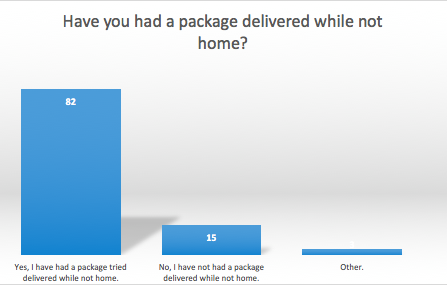
\includegraphics[width=300]{pics/packagedeliverednothome.png}
  \caption{Packagedelivered while not at home [Bilag 1]}
  \label{fig: survey1}
\end{figure}

 83\% of the participants in our survey have experienced that while they were at work a delivery company have attempted to deliver a package to their house as seen in Figure \ref{fig: survey1}. This becomes a problem for not only the customer that has to agree upon a new delivery date or pick up the package at a pick-up point. And the delivery company has spend time driving to a customer that is not available, which means they have spend resources on a delivery that might happen again at a later date. This system is far from optimized and while some customers choose to wait at home the whole day from work, most do not have that option and the delivery attempts to their homes will be unsuccessful.

\begin{figure}[H]
  \centering
  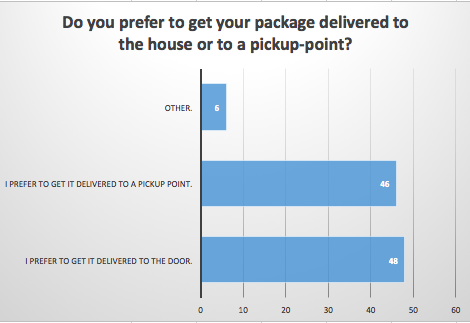
\includegraphics[width=300]{pics/houseorpickuppoint.png}
  \caption{Do you prefer house or pick-up point. [Bilag 1]}
  \label{fig: survey2}
\end{figure}

In the survey the preferred way to get a package delivery is close to evenly split. With a 46\% preferring to pickup the package at a shop or other package pick-up points. While 48\% prefer to get it delivered to their home as you see in Figure \ref{fig: survey2}. 
This is often reasoned to the point that they are never home when the package is getting delivered, as almost 90\% of the people that preferred a pick-up point says it is because they expect not to be home when the package is delivered. And it would be easier for them to pick it up on the way to or from work or class. Instead of staying home a full day because of the lack in proper information about the time of the day the package will get delivered.


\begin{figure}[H]
  \centering
  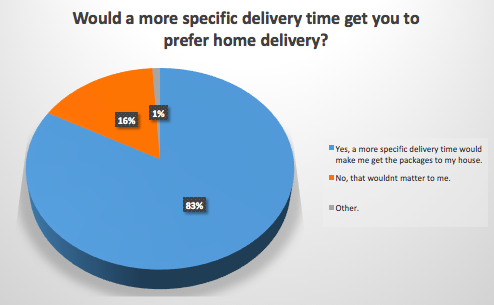
\includegraphics[width=300]{pics/morespecific.png}
  \caption{Would a more specific time help with being home. [Bilag 1]}
  \label{fig: survey3}
\end{figure}

 With a narrower time frame the delivery companies could make sure people are home when a package delivery is attempted. Because the receiver only have to be home for maybe an hour or two instead of a whole day.\\\hspace*{5 mm}
 83 \% of people would rather have their package delivered to their doorstep if they could choose a time frame of the day as shown in Figure \ref{fig: survey3}.
 In those 83 \% there is 26 \% that preferred to get their package send in to a pickup point, but with a more specific time frame it would make them switch their stance, this is over half that would consider changing the way they get a package delivered. \\

The hundred people asked in our survey would mostly want their package delivered to their home address, if the possibility for a more narrow time frame or even being a part of picking the time themselves. This could solve problems for both parties of package delivery. The customers would have a better chance of being home when their package are getting delivered, and the delivering companies would not have to make as many drives to people whom are not home. 


\section{Last Mile Delivery}
The last mile delivery section will we look into different reasons to why it is this specific part of the route that focus have been put on. And why an optimization in the last mile would be a great help for delivering companies.

Last mile delivery is a logistics term and refers to the final step of the order being dispatched from a transportation hub to the customer receiving their package. 
Last mile delivery has become a problem for couriers as this part of the supply chain is often less efficient than freight transporting goods by container ships, train or trucks. Transporting goods in freight is very straightforward, however once the goods arrive at the transportation hubs they must then be transported to their final destination. Unlike freight transportation which can contain packages in large bulks and therefore lower the overall cost per package, where the last mile often demands one or two packages to get delivered per house, which means a less time efficient way of getting the packages out, and the constant demand from the public about a faster delivery puts a constant pressure on the delivery companies. 
\begin{figure}[H]
  \centering
  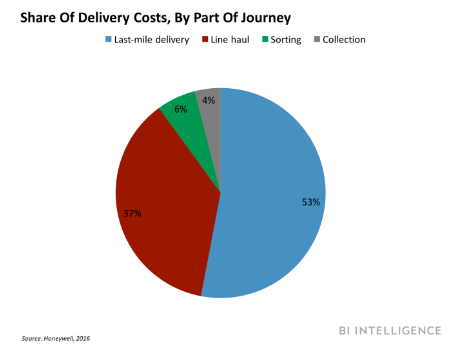
\includegraphics[width=345]{pics/lastmile.png}
  \caption{The different legs in delivery and their weight\cite{lastmile2}.}
  \label{fig: LastMile}
\end{figure}
As seen in Figure \ref{fig: LastMile}, the last mile in delivery takes up over 50\% of the cost, and is a place where an optimization could give large cuts in the cost. 
Therefor there have been looks into a way to optimize this by the industry, and many options are being considered.\cite{lastmile}
Where improved tracking and better communication with the customer tops the list of things to be developed in the future.
The increase in e-commerce has also contributed to this problem, as people are buying more products online and demand fast shipping times. Increased e-commerce means more packages being sent, and couriers are now searching for new ways to transport goods as traditional transportation methods aren't successful anymore\cite{lastmile}. 

There have been a great deal of focus on the last mile from companies, because the great costs of the last leg of the delivery, and while the e-commerce is rising the need of optimization will do the same. \\\hspace*{5 mm}




\section{Part conclusion}
% skal afrunde afsnitene omkring kundetilfredshed, konkludere at der er et problem. Overgang til afsnit der omhandler økonomi.
The survey in customer convenience show a trend in the initial problem...



%SUB QUESTION 2: Is it beneficial for companies to focus on customer satisfaction?
\section{Economy}
Economy is an important segment for all companies \cite{economyimportance}. This includes the top distribution companies in Denmark, which this section focuses on, PostNord, GLS and UPS\cite{okonomiskansvar, Postnordmiljoansvar, ThinkGLS}. Delivering a high amount of packages in short time and using an optimized route supports the foundation of a strong economy.\\\hspace*{5mm}
Furthermore an optimized, and thereby shorter, route saves fuel and prevents further environmental pollution. PostNord, GLS and UPS all intents to pollute as little as possible\cite{Postnordmiljoansvar, ThinkGLS, UPSmiljo}.


\subsection{Fuel economy}
%Nævn miljø
%fokus på besparelser i forhold til sparede km(når man dropper en levering pga de ik er hjemme.)
Postnord is using the their environment accountability to reduce the general load of CO2 they use there environmental policy to get better economics sustainability as they use this as a marketing strategy to getting more customers whom also focus on the environment \cite{Postnordmiljoansvar}. 
While GLS will also benefit on lowering the expensive on there delivery time with more packages delivered, both economic and environment they will benefit on getting a better and more optimized route because they also have a environmental plan they are trying to live by called Thinkgreen \cite{ThinkGLS}. 
the understanding of Thinkgreen is to find a better way both economically and environmentally better way of delivery more packages to customers\cite{ThinkGLS}. 
Both by getting cheaper and more reliant fuel, but also by driving "better" trucks which drives longer pr. mile of fuel. 
Last is UPS and GLS which still have a lot to gain on the Danish market because they are lesser known and not as big as Postnord in Denmark which we can see out of there net revenue is not as big as Postnord\cite{Postnordregnskab, GLSregnskab, UPSregnskab}.
its important for all companies to have a good sustainable economics. 
Also to see if companies can afford too focus only on the customers needs.
%Translate ALLE valuta til danske kroner.
%Fokuser på Post nord og UPS og GLS


\section{The benefits of prioritizing customers}
%mulig indledning også
Attracting new customers is the main goal for every company and is the foundation for having returning customers. Customers who repeatedly visits a specific company or brand spend 67\% more money than customers who visit for the first time\cite{BainAndCompany}. Customers who have been returning to the same company or brand two times refer an average of 3 people to the company whereas customers who have been returning to a company ten times are in general referring an average of seven people\cite{BainAndCompany}, which is seven new customers who will have the potential of referring an average of seven people each. A referred customer will on average spend 50\% more money than a new customer might\cite{BainAndCompany}.
New customers cost about 20-40\% to obtain so it is cheaper for a company to maintain current customers than reaching out for new ones\cite{E-loyalty}.
In the light of this it can be concluded that it is important for a business to have returning customers because returning customers and a great customer satisfaction are a much more profitable way of doing business than only relying on new customers.
Online retailers who have returning customers will eventually be more profitable than their competitors, because returning customers refer more friends, generally spends more and are cheaper for the company to retain\cite{BainAndCompany}\cite{E-loyalty}.

 

\section{Part conclusion}

%Finde en balance mellem besparelser og kundetilfredshed.


%SUB QUESTION 3: How does existing methods handle the problem?

\section{Top delivery companies and their methods}
%Ændre titel
%Virker som intro til besvarelse af subquestion 3.
Receiving mail is an everyday phenomenon. Getting packages delivered to either a home address or a parcel box on a weekly basis is becoming more common. In a research conducted by the danish ministry of transport, one in four people receive packages ordered online up to three times a month and around two thirds receives one or more packages every quarter of the year\cite{reportDKpakketjenester}. How these people choose to get their packages delivered varies depending on their place of residence. People living in big cities shows a tendency to receive packages more frequently than ruralites \cite{reportDKpakketjenester}. Getting packages delivered to home addresses is still the most used method by both city residents and ruralites(kilder). Most cities offers other alternatives such as parcels boxes, which stores the package for you to pick up, while rural areas are more reliant on home deliveries due to longer travel times to the nearest pick-up points.\cite{reportDKpakketjenester}.\\\hspace*{5 mm}
Parcel boxes are getting used more. Usage have risen 10\% from 2015 to 2018 while delivery to home addresses have fallen 7\% in the same time period. Elderly people above the age of 65 is more likely to use home delivery while the younger age groups and families with children are more frequent users of the parcels boxes and pick up points\cite{FDIHyearreport}.
(Spørgeskema op mod dette evt.).

Postnord and GLS both provide their own solutions to comprehend the delivery requirements giving by the customers, but their solutions only provide the customers with influence by some degree. Both PostNord and GLS provide a service that let the customer choose where on their address that the distributor is allowed to put it. This gives the customer the freedom of not needing to be home at the time of delivery but also presents a problem. The customer is held fully responsible if the package is either lost or stolen from their address after it has been delivered by the distributor\cite{postnordoptions}\cite{glsoptions}. Furthermore this service is not optimal if living in an apartment complex where no secluded areas are available for the package to be placed. As mentioned earlier, parcels boxes is widely used by the danish population and both PostNord and GLS delivers to these while also being able to drop the package of at a pick up point either chosen by the customer or closest in proximity if nothing has been specified by the customer \cite{postnordoptions}\cite{glsoptions}.

In all the cases of delivery options giving by the distributor described above, none of them gives the customer full control of the delivery time. They provide solutions that involves the customer in risking losing their package\cite{Pakketyveri} GLS even provides the customer with the option of what day they want the package delivered, but this still forces the customer to be at home at the time of delivery if they want the package without risking it being stolen if placed somewhere on the address\cite{Pakketyveri}. \\


New transportation technologies are being developed to help lower the cost and increase the efficiency of last mile delivery. Companies are looking to drones, droids, and autonomous delivery vehicles. By using semi and fully autonomous delivery vehicles in cities couriers will be able to reduce delivery costs by 10 to 40\% while also reducing their CO2 emissions greatly by using electric vehicles \cite{FastForwardingLast-mileDelivery}. \\




\section{UPS Orion}
This section will focus on the importance of optimization software solutions. Through information obtained about United Postal Service's (UPS) route planning software Orion (On-Road Integrated Optimization and Navigation)\\

With Orion UPS searches to optimize the distance, time and fuel the UPS drivers uses on their routes. Orion takes into consideration the start time, commit time (the estimate for when the package is delivered), pick up windows (the window of time when the driver can pick up packages that needs to be shipped) and special customer requests. When Orion calculates the most cost effective route for the driver to use \cite{orionbackgrounder}.\hspace*{5mm}

The development of the algorithm which is used in Orion, started in 2003 and lasted until 2009. UPS then began testing it in 8 of their sites in 2010. The algorithm for Orion is according to UPS around 1000 pages of code. This comes to show the magnitude of the optimization there is to package delivery \cite{orionbackgrounder}.\hspace*{5mm}

According to UPS the implementation of Orion saves them around 161 million driven kilometers (100 million miles) per year. This means UPS can save around 37,8 million liters (10 million gallons) of fuel a year. UPS’s own results have showed that a reduction of just 1 mile a day per driver can save UPS around 331 million Danish kroner in a year. UPS also tells that Orion can bring benefits to the customers, by allowing the customers to choose their preferences for the packages they receive \cite{orionbackgrounder}.  

\section{Impact of traffic related instances}

Delivery companies often have problems specifying the time in which customers receive their packages that results in them only telling you a specific day. A big reason to this is the uncertainty when it comes to traffic. Data from Open Data DK shows the traffic peaks on roads in Aalborg\cite{traficcount}. 

This report examines the data for six streets; Karolinelundsvej, Kastetvej, Sohngårdsholmsvej, Vesterbro, Østerbro, and Østre Alle\cite{traficcount} as these are some of Aalborgs connecting roads and  are therefore heavily trafficated doing the day. By examining the data it can be concluded that the traffic congestion on these streets follow the work hours in Denmark. The beginning peak time on all six streets in the morning are 07:23 on average, this is when people start their commute to work. And the beginning of the peak time in the afternoon are 15:05 on average which is close to peoples commute from their work to their home.\hspace*{5mm}

Thereby it can be concluded that the most optimal time of the day to deliver packages, are in the hours between 8 in the morning and 15 in the afternoon, which is when people are at work. As seen in the user survey, people choose to get their packages delivered to a package pickup point. Because they might not be home in these hours, therefore the most convenient and efficient time of day for the delivery company, would be before peak hours in the morning, or after peak hours in the afternoon. Nonetheless the delivery companies will have to take the peak hours into consideration as they can greatly impact the delivery time estimate if not calculated for.\\

\section{Algorithm}

In this chapter The travelling sales man problem and two of the algorithms used to solve it will be described. To understand why there is a problem in creating routes for package delivery. And what have been done in effort of finding the most optimal route.\\ 

The package delivery problem is a variation of the travelling sales man problem. The travelling salesman problem revolves around a salesman, who have to visit n number of cities, and then return home to his own town. The best solution for his route is therefore a Hamiltonian which is a route where he only visits every city once before he travels home to the starting point.\hspace*{5mm}

The travelling salesman problem is a well known problem in computer science and especially graph theory because it is known to be NP-complete. As it is a multigraph where there usually are at least two ways to get to the next city. And therefore there will be at least two edges to every vertice\cite{tsp}.

\begin{figure}[H]
  \centering
  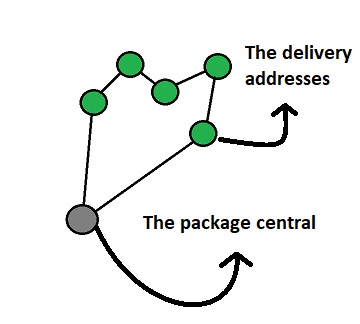
\includegraphics[width=300 pt]{pics/tsp.jpg}
  \caption{The Travelling Salesman Problem}
  \label{fig: The Travelling Salesman Problem}
\end{figure}\textbf{}

This is also the issue in the delivery problem, as there in most cases will be more than one way to reach each address. An example of this can be seen in Figure 2.7 which is an example where the delivery driver needs to travel from the package central to 5 different delivery addresses. In the delivery problem version of the travelling salesman problem it will be the route where the delivery truck does not have to visit or cross a street more than once\cite{tsp}. There has not been found an algorithm which can solve the problem, the best solution for the problem were created by Keld Helsgaun from Roskilde University\cite{keld}. Helsgaun created an algorithm which makes a route that is only 0.0474\% longer than the optimal route for the problem\cite{tsp2}.\\

Due to the fact that the travelling salesman problem have not been solved. Each delivery company have different computer programs and algorithms they use. Even businesses who only focus on package routing have been started, an example of this is Routific who has created a piece of software they sell to companies who needs routing for delivery their delivery services\cite{routific}.         


\subsection{Genetic algorithm}
One way of finding routes for the travelling salesman problem is a genetic algorithm. The idea behind genetic algorithm comes from Charles Darwin's theory of evolution and is based on the survival of the fittest principal. The algorithm therefore makes the strongest element in the generation the father for the next generation. To solve the problem of package delivery you start with a generation of random routes. Each of the routes gets assigned a fitness value depending on how close it is to the goal that is the best route/shortest route. The route with the best score gets to be the father of the next generation of routes. This selection keeps happening until the best route have been discovered or made. Or at least until the fitness score gets balanced and does not improve further in the next generations\cite{geneticalg}.

\subsection{Greedy algorithm}
Another way of finding routes for TSP is by using a greedy algorithm. The greedy it always takes the nearest city which has not been visited, this creates the most direct route between the cities, this could create the best solution locally and is expected to have a result on a larger scale that is within a limited range of the optimized solution. While this outcome is a faster route than a random picked route, it is not in all cases the most optimized route\cite{solvingcdp}.

\section{Part Conclusion}
So to conclude the package delivery problem 

\chapter{Problem Statement}


\chapter{Problem Definition}

Draft // The delivery period for the customers are too big. \\
Can be solved with a piece of software that can optimize package delivery so that the customer has a better idea of when the packages will arrive at their doorstep.

\chapter{DRAFTS}
As per the 1st January 2017 the Danish Customs and Tax Administration (SKAT) removed the special rules for e-commerce companies usage of the taxation law 
Which means that ordering things from the internet, will be cheaper, and is therefore a win for the industries, both the package delivery industry, and the E-business. And because there were no tax obligations on the “Postal Offices” delivering of packages, since 1989, they have had big advantages, in package delivery since they could deliver their packages cheaper than the other package delivery companies\cite{ikkemeremoms}.

%Kildeliste
\bibliography{kilder}


\end{document} 